% \documentclass[11pt, usenames, dvipsnames, handout]{beamer}
\documentclass[11pt, usenames, dvipsnames]{beamer}


%%%%%%%% tema e cor %%%%%%%%
\mode<presentation> {
\usetheme{PaloAlto}
\setbeamerfont{section in sidebar}{size=\fontsize{5}{5}}
\setbeamerfont{subsection in sidebar}{size=\fontsize{3}{5}}
\setbeamerfont{section in sidebar shaded}{size=\fontsize{2}{4}}
}

\usepackage[utf8]{inputenc}
\usepackage{graphicx} 
\PassOptionsToPackage{dvipsnames}{xcolor}
\usepackage{booktabs} 



\institute[HUJI] 
{
%================= logos no meio =====================
\vspace*{-0.35cm}
\hspace*{0.25cm}~%
\vspace*{0.35cm}\\
Introduction to Machine Learning (67577)}
\date{\today}

\AtBeginSection[]
{
\begin{frame}
\frametitle{Outline}
\tableofcontents[currentsection]
\end{frame}
}

% \usecolortheme{crane}
\newtheorem{exercise}{Exercise}
\newtheorem{remark}{Remark}
\newtheorem{claim}{Claim}

\let\OLDremark=\remark
\def\remark{%
  \setbeamercolor{block title}{bg=Gray}%
  \setbeamercolor{block body}{fg=black,bg=white!80!Gray}\OLDremark
}
\let\OLDtheorem=\theorem
\def\theorem{%
  \setbeamercolor{block title}{bg=black!65!brown}%
  \setbeamercolor{block body}{fg=black,bg=white!80!brown}\OLDtheorem
}
\let\OLDclaim=\claim
\def\claim{%
  \setbeamercolor{block title}{bg=black!60!red}%
  \setbeamercolor{block body}{fg=black,bg=white!85!red}\OLDclaim
}
\let\OLDcorollary=\corollary
\def\corollary{%
  \setbeamercolor{block title}{bg=black!65!orange}%
  \setbeamercolor{block body}{fg=black,bg=white!80!orange}\OLDcorollary
}
\let\OLDproof=\proof
\def\proof{%
  \setbeamercolor{block title}{bg=Dandelion}%
  \setbeamercolor{block body}{fg=black,bg=white!80!yellow}\OLDproof
}
\let\OLDexercise=\exercise
\def\exercise{%
  \setbeamercolor{block title}{bg=OliveGreen}%
  \setbeamercolor{block body}{fg=black,bg=white!80!LimeGreen}\OLDexercise
}
\let\OLDsolution=\solution
\def\solution{%
  \setbeamercolor{block title}{bg=BurntOrange}%
  \setbeamercolor{block body}{fg=black,bg=white!80!Dandelion}\OLDsolution
}
\let\OLDlemma=\lemma
\def\lemma{%
  \setbeamercolor{block title}{bg=Orchid}%
  \setbeamercolor{block body}{fg=black,bg=white!80!Purple}\OLDlemma
}


\addtobeamertemplate{navigation symbols}{}{%
    \usebeamerfont{footline}%
    \usebeamercolor[fg]{footline}%
    \hspace{1em}%
    \insertframenumber/\inserttotalframenumber
}

%%%%%%%% titulo e subtitulo %%%%%%%%
\title[Introduction to Machine Learning (67577)]{Introduction to Introduction to Machine Learning: Probability} 

%%%%%%%% nome dos autores %%%%%%%%
\author[Gad Zalcberg]{Gad Zalcberg} 



\begin{document}
\titlepage 
\newcommand{\cD}{\mathcal{D}}
\newcommand{\bE}{\mathbb{E}}
\newcommand{\prob}{\mathbb{P}}


%%%%%%%% slides %%%%%%%%
\section{Probability: Recap} 
\subsection{Probability Space}
\begin{frame}{Sample space}

    \begin{definition}[Sample Space]
    The \textbf{sample space} $\Omega$ of an experiment or random trial is the set of all possible outcomes or results of that experiment.
    
    $\omega\in\Omega$ denotes a single outcome.
    \end{definition}
    
    \pause
    
    Examples:
    \begin{itemize}
    \item Coin toss: $\Omega=\left\{ H,T\right\} $

    \pause
    \item Toss a coin until heads comes up: $\Omega=\left\{ T^{n-1}H:n\in\mathbb{N}\right\} $
    
    \pause
    \item Rolling two (distinguishable) dice: $\Omega=\left\{ 1,\dots,6\right\} ^{2}$
    What will be the sample space if the dice are indistinguishable? $\Omega=\left\{ \left(i,j\right):1\le i\le j\le6\right\} $
    \pause
    \item Waiting time at the post office: $\Omega=[0,\infty)$
\end{itemize}
    
\end{frame}

\begin{frame}{Events}
\begin{definition}[Events]
An \textbf{event} $A$ is any subset of possible outcomes, $A\subseteq\Omega$.
\end{definition}
\pause
Quick reminder:
\begin{itemize}
\item $A^{c}$ (or sometimes $\overline{A}$) denotes the \textit{complement} of $A$, $A^{c}=\Omega\backslash A$ . In other words, $A^{c}$ is the event that $A$ did not occur. 
\pause
\item We say that $A$ and $B$ are \textit{disjoint} \textit{events} if $A\cap B=\emptyset$.
\pause
\item $\Omega$ and $\emptyset$ are also events. If $A$ and $B$ are two events, then $A\cup B$ is also an event, and so is $A\cap B$. 
\end{itemize}
\end{frame}

\begin{frame}{Probability Space}

\begin{definition}[Probability Space]
A probability space is a tuple \footnote{For our needs this simple and intuitive definition is sufficient, though richer definitions exist.} $(\Omega, \mathcal{D})$ where $\Omega$ is a \emph{sample space} and $\mathcal{D}:2^{\Omega}\rightarrow\mathbb{R}$ is a probability function such that 
% you might want to remind them what is 2^Omega

\begin{enumerate}
\item $\mathcal{D}(\Omega)=1$
\item for all $\omega\in\Omega,;\cD(\omega)\in[0,1]$
\item for all $A,B\subseteq\Omega$ such that $A\cap B=\emptyset,$ we have $\cD(A \cup B)=\cD(A)+\cD(B).$
\end{enumerate}
\end{definition} 
\pause
\begin{example}
Suppose we throw two fair dice, $\Omega=\left\{ 1,\dots,6\right\} ^{2}$ and $\cD\left(\left(i,j\right)\right)=\frac{1}{36}$
\end{example}

\end{frame}

\begingroup
\small% \small in 11pt base font is 10pt
\begin{frame}{Exercise}

\begin{exercise}
For all $A,B\subseteq\Omega$: $$\cD(A\cup B)=\cD(A)+\cD(B)-\cD(A\cap B)$$
\end{exercise}
\pause
\begin{solution}
We have:
\begin{align*}
    A\cup B=&(A\setminus B)\cup(B\setminus A)\cup(A\cap B)\\
    A=&(A\setminus B)\cup(A\cap B) \\
    B=&(B\setminus A)\cup(A\cap B)
\end{align*}
\pause
\begin{align*}
    \cD(A\cup B)= & \cD(A\setminus B)+\cD(B\setminus A)+\cD(A\cap B)\\
    =&\cD(A)-\cD(A\cap B)+\cD(B)-\cD(A\cap B)+\cD(A\cap B)    
\end{align*}
\end{solution}
\end{frame}
\endgroup
\begin{frame}{Independence}
\begin{definition}[Independence]
$A,B\subseteq\Omega$ are called \emph{independent} if: $$\cD(A\cap B) =\cD(A)\cdot\cD(B)$$
\end{definition}
\pause
\begin{exercise}
If $A$ and $B$ are independent then $A$ and $B^c$ are also independent. 
\end{exercise}
\pause
\begin{solution}
$$\cD(A)=\cD(A\cap B)+\cD(A\cap B^c)=\cD(A)\cdot\cD(B)+\cD(A\cap B^c)$$ 
\pause
$$\Rightarrow\cD(A\cap B^c)=\cD(A)(1-\cD(B))=\cD(A)\cdot\cD(B^c).$$
\end{solution}
\end{frame}

\begingroup
\footnotesize% \small in 11pt base font is 10pt
\begin{frame}{Union Bound}[The Union Bound]
\begin{lemma}  \label{lem:unionBound} Let
$(\Omega, \cD)$ be a probability space. The probability function is \emph{sub-additive}, i.e., for any sequence $(A_k)$ of events,
$$\cD(\cup_{k=1}^\infty A_k) \le \sum_{k=1} ^\infty \cD(A_k)$$
\end{lemma}
\pause
\begin{proof}
Let $B_1=A_1$. For each $k \in \{2,3,\ldots\}$, let $B_k = A_k
\setminus \cup_{i=1}^{k-1} A_i$. \\
\pause
Note that the $B_1...B_k$ are disjoint, and $\cup_{i=1}^k A_i=\cup_{i=1}^k B_i$. \\
\pause
Also, since $B_k\subseteq A_k$, $\cD(B_k) \le \cD(A_k)$ for every $k \in \mathbb{N}$.\\
\pause
It follows by the countable additivity of $\cD$ that:
$$\cD(\cup_{k=1}^\infty A_k) = \cD(\cup_{k=1}^\infty B_k) = \sum_{k=1}
^\infty \cD(B_k) \le \sum_{k=1}
^\infty \cD(A_k) 
$$
\end{proof} 
\end{frame}
\endgroup
\subsection{Random Variables}

\begin{frame}{Random Variables}

\begin{definition}[Random Variable]
Given a probability space $\left(\Omega,\cD\right)$, a \textit{real-valued
random variable} is a function $X:\Omega\rightarrow\mathbb{R}$.
\end{definition}

\pause

\begin{remark}
Any function $g\left(X\right)$ of a random variable is also a random
variable (for instance $X^{2}$, $sign\left(X\right)$, etc.).
\end{remark}

\pause

For a discrete $\Omega$ we define the \textbf{\textit{probability
mass function}} of $X$ (a \textit{discrete RV}) as 
\[
\cD\left(\left\{ X=x\right\} \right)=\sum_{\omega:X\left(\omega\right)=x}\cD\left(\omega\right)
\]
Instead of writing $\cD\left(\left\{ X=x\right\} \right)$ we usually
write $\cD\left(x\right)$.
\end{frame}

\begin{frame}{Random Variable - Example}
\begin{example}
A fair coin is tossed twice. The probability space  is $\Omega=\left\{ T,H\right\} ^{2}$
and $\cD\left(\omega\right)=\frac{1}{4}$. Let $X$ be the number of
times heads came up. In this case we have $\mathcal{X}=\left\{ 0,1,2\right\} $
and
\[
\cD\left(x\right)=\begin{cases}
\frac{1}{4} & x=0,2\\
\frac{1}{2} & x=1\\
0 & \mbox{else}
\end{cases}
\]
\end{example}
\end{frame}

\begin{frame}{Continues RV}
For a continuous $\Omega$ - we say that $X$ is a \textit{continuous
RV} if we can write for every $D\subset\mathbb{R}$ 
\[
\cD\left(X\in D\right)=\int_{D}f\left(x\right)dx
\]
\pause

In particular, this means we can write for every $\left[a,b\right]\subset\mathbb{R}$
\[
\cD\left(X\in\left[a,b\right]\right)=\int_{a}^{b}f\left(x\right)dx
\]

\pause

Note, that for any $a\in\mathbb{R}$:  $\cD\left(X=a\right)=\int_{a}^{a}f\left(x\right)dx=0$.

\pause

The function $f$ is called the \textbf{\textit{probability density
function }}\textbf{(PDF)} of $X$. 

\pause

Note that - 
\begin{itemize}
\item $f\left(x\right)\ge0$
\item $\int_{-\infty}^{\infty}f\left(x\right)dx=1$ 
\item $f\left(x\right)$ is not a probability, and it could be that $f\left(x\right)>1$.\\
\end{itemize}

\end{frame}

\subsection{Expectation and Variance}
\begin{frame}{Expectation}
\begin{definition}[Expectation]
The \textbf{\textit{expected value}} of a random variable
$X$ is
\[
\bE\left[X\right]=\sum_{x\in\mathcal{X}}x\prob\left(x\right)\qquad\mbox{or}\qquad \bE\left[X\right]=\int_{-\infty}^{\infty}xf\left(x\right)dx
\]
\end{definition}

\pause

Properties:
\begin{itemize}
\item $\bE\left[g\left(X\right)\right]=\sum g\left(x\right)\cD\left(x\right)$,
\pause
\item $\bE\left[c\right]=c$
\pause
\item Linear: $\bE\left[aX+Y\right]=a\bE\left[X\right]+\bE\left[Y\right]$
\pause
\item If $X$ and $Y$ are independent then $\bE\left[XY\right]=\bE\left[X\right]\bE\left[Y\right]$\\
Since: $\bE[XY]=\sum\cD(X=x,Y=y)x\cdot y = \sum_{x,y}\cD(x)\cD(y)xy=\bE[X]\bE[Y]$
\end{itemize}
    
\end{frame}

\begin{frame}{Variance}

\begin{definition}[Variance]
Let $X$ be a RV with $\bE\left[X\right]=\mu$, then the \textbf{\textit{variance}}
of $X$ is 
$$V\left(X\right)=\bE\left[\left(X-\mu\right)^{2}\right]$$
The \textbf{\textit{standard deviation}} is defined as $\sigma=\sqrt{V\left(X\right)}$.
\end{definition}
\pause

Properties of the variance:
\begin{itemize}
\item $V(X)\geq0$ , $V(X)=0\,\iff\,X$ is a constant.
\pause
\item $V\left(X\right)=\bE\left[X^{2}\right]-\bE^{2}\left[X\right]$
\pause
\item $V(aX+b)=a^{2}V(X)$
\pause
\item $V(X+Y)=\bE\left[\left(X+Y-\bE(X)-\bE(Y)\right)^{2}\right]=V(X)+V(Y)+2\overbrace{\bE\left[\left(X-\bE[X]\right)\left(Y-\bE[Y]\right)\right]}^{Cov\left(X,Y\right)}$
\pause
\item If $X_{1},\dots,X_{n}$ are independent then $V\left(\sum X_{i}\right)=\sum V\left(X_{i}\right)$\end{itemize}


\end{frame}

\begin{frame}{Variance - Exercise}
\begin{exercise}
Let $Z$ be a Bernoulli random variable. Calculate $Var[Z].$ 
\end{exercise}
\pause
\begin{solution}
$Var[Z]=E[Z^2]-E^2[Z]=p-p^2=p(1-p).$
\end{solution}
\end{frame}

\begin{frame}{Covariance}

\begin{definition}[Covariance]
The \textbf{\textit{covariance}} of $X$ and $Y$ is
\[
Cov(X,Y)=\bE\left[\left(X-\bE[X]\right)\left(Y-\bE[Y]\right)\right]=\bE\left[XY\right]-\bE[X]\bE[Y]
\]

\end{definition}

\pause
Properties:
\begin{itemize}
\item $Cov(X,Y)=Cov(Y,X)$
\pause
\item $Cov(aX+b,cY+d)=acCov(X,Y)$
\pause
\item $Cov(X,X)=V(X)$
\end{itemize}
    
\end{frame}

\begingroup
\small% \small in 11pt base font is 10pt

\begin{frame}{Variance - Example}
\begin{example}
Find the mean and variance of $X\sim U\left(\left[a,b\right]\right),$ where $U[a,b]$ is the uniform distribution on $[a,b].$
\begin{eqnarray*}
\bE\left[X\right] & = & \frac{1}{b-a}\int_{a}^{b}xdx=\frac{1}{2\left(b-a\right)}\left(b^{2}-a^{2}\right)=\frac{b+a}{2}\\
\pause
\bE\left[X^{2}\right] & = & \frac{1}{b-a}\int_{a}^{b}x^{2}dx=\frac{1}{3\left(b-a\right)}\left(b^{3}-a^{3}\right)=\frac{b^{2}+ab+a^{2}}{3}\\
\pause
V\left(X\right) & = & \frac{b^{2}+ab+a^{2}}{3}-\frac{\left(b+a\right)^{2}}{4}=\frac{\left(b-a\right)^{2}}{12}
\end{eqnarray*}
\end{example}

\end{frame}
\endgroup
\section{High Dimensional Distributions}

\begingroup
\footnotesize% \small in 11pt base font is 10pt
\begin{frame}{Sample Variance/Covariance}
\begin{definition}[Sample Variance]
    Assume $\{x_{1},x_{2},\ldots ,x_{n}\}$ is a sample (formally, realizations from a random variable X) and ${\overline {x}}$ is the sample mean, than the estimator of the variance is given by:
$$\sigma^2_x = \frac{1}{n-1} \sum^{n}_{i=1}(x_i- \bar{x})^2$$
\end{definition}
\pause

\begin{definition}[Sample Covariance]
    Assume $\{x_{1},x_{2},\ldots ,x_{n}, y_{1},y_{2},\ldots ,y_{n}\}$ is a sample, and ${\overline {x}}$, ${\overline {y}}$ is the sample mean, than the estimator of the covariance $\sigma\left(x,y\right)$ of two random variables X and Y is given by:
$$\sigma(x, y) = \frac{1}{n-1} \sum^{n}_{i=1}{(x_i-\bar{x})(y_i-\bar{y})}$$

\end{definition}
\end{frame}
\endgroup

\subsection{Covariance Matrix}
\begin{frame}{Covariance Matrix}
\begin{definition}[Covariance Matrix]
    Assume $\{\textbf{x}_{1},\textbf{x}_{2},\ldots ,\textbf{x}_{n}\}$ is a sample, for each $i\in[n]:\; \textbf{x}_i\in\mathbb{R}^d$, and assume ${\overline {\textbf{x}}}$ is the sample mean, than the estimator of the variance is $C\in\mathbb{R}^{d\times d}$ where $C_{ij}=\sigma\left(x^{i},x^{j}\right)$.
\end{definition}
\pause
Note: 
\begin{itemize}
    \item The calculation of the covariance matrix can be also expressed as:
$$C = \frac{1}{n-1} \sum^{n}_{i=1}{(X_i-\bar{X})(X_i-\bar{X})^T}$$
And for a data set with zero mean: $C = \frac{XX^T}{n-1}$
    \pause
    \item The covariance matrix is symmetric, since $$\sigma\left(x^{j},x^{i}\right)=\sigma\left(x^{i},x^{j}\right)$$
\end{itemize}
\end{frame}

\begingroup
\small% \small in 11pt base font is 10pt
\begin{frame}{Numerical Example}
\begin{exercise}
let $X=\left(\begin{array}{ccc}
150 & 170 & 184\\
45 & 74 & 79
\end{array}\right)$ be samples of hight and weight of 3 different people where $X_{1i}$ is the hight and $X_{2i}$ is the weight of the i'th man. calculate the covariance matrix of the sample.
\end{exercise}
\pause
First of all we will make the the data centered:\\
We have: $\bar{x_1}=168$ and $\bar{x_2}=66$, so $$X_{centered}^{T}=X^T-\bar{x}=\left(\begin{array}{cc}
150 & 45\\
170 & 74\\
184 & 79
\end{array}\right)-\left(\begin{array}{c}
168,\;66\end{array}\right)=\left(\begin{array}{cc}
-18 & -21\\
2 & 8\\
16 & 13
\end{array}\right)$$
\pause
and: 
$$
cov(X)=\frac{X_{centered}X_{centered}^{T}}{3-1}=\left(\begin{array}{cc}
292 & 301\\
301 & 337
\end{array}\right)
$$
\end{frame}
\endgroup
\subsection{Linear Transformations of the Data Set}

\begingroup
\footnotesize% \small in 11pt base font is 10pt
\begin{frame}{Two Dimensional Example: Uncorrelated}
Lets focus on the two-dimensional case (it can be easily generalized to more dimensional data). covariance matrix for two dimensions is given by:
$$C = \left( \begin{array}{ccc}  \sigma(x, x) & \sigma(x, y) \\  \sigma(y, x) & \sigma(y, y) \end{array} \right)$$
\pause
First we will take random (normal distribution) points with mean values $\bar{x}=\bar{y}=0$ and unit covariance $\sigma\left(x\right)=\sigma\left(y\right)=1, \; \sigma\left(x,y\right)=\sigma\left(y,x\right)=0$ (also called white noise):
\pause

\begin{figure}[h!]
  \centering
    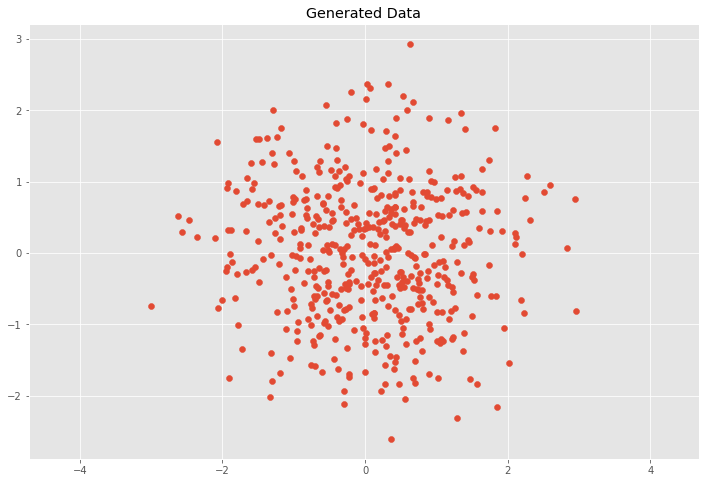
\includegraphics[scale=0.2]{uncorrelated.png}  
   \caption{Uncorrelated Variables}
\end{figure}
\end{frame}

\begin{frame}{Two Dimensional Example: Scaling}
We will transform our data with the following scaling matrix:
$$S = \left( \begin{array}{ccc}  s_x & 0 \\  0 & s_y \end{array} \right)$$
(transformation simply scales the x and y components by multiplying them by $s_x$ and $s_y$ respectively).\\
\pause
The covariance matrix C of our transformed data set will be:
$$C = \left( \begin{array}{ccc}  (s_x\sigma_x)^2 & 0 \\  0 & (s_y\sigma_y)^2 \end{array} \right)$$
\pause

\begin{figure}[h!]
  \centering
    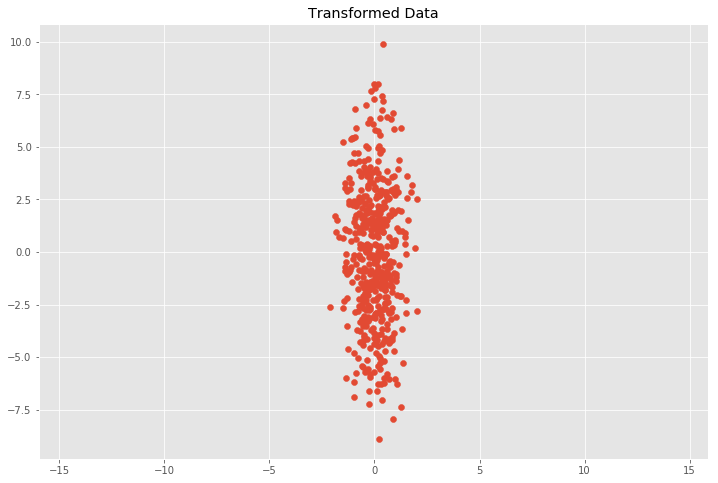
\includegraphics[scale=0.2]{uncorrelated_scaled.png}  
   \caption{Uncorrelated Scaled Variables}
\end{figure}
\end{frame}
\endgroup
\begin{frame}{Two Dimensional Example: Scaling + Rotation}
    Let $R\in\mathcal{O}_2$ a rotation matrix given by:
$$R = \left( \begin{array}{ccc}  cos(\theta) & -sin(\theta) \\  sin(\theta) & cos(\theta) \end{array} \right)$$ where $\theta$ is the rotation angle. And define $$T = RS$$ 
\pause
The transformed data is then calculated by $Y=TX=RSX$ and the covariance matrix are:    $$YY^T=RSX(RSX)^T=RSXX^TS^TR^T=RSCS^TR^T$$
$$=R\left( \begin{array}{ccc}  (s_x\sigma_x)^2 & 0 \\  0 & (s_y\sigma_y)^2 \end{array} \right)R^T
$$
\end{frame}

\begin{frame}{Two Dimensional Example: Scaling + Rotation}
\begin{figure}[h!]
  \centering
    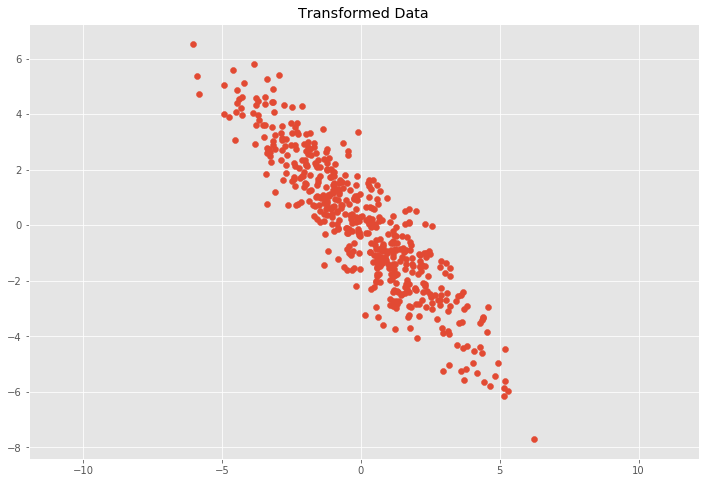
\includegraphics[scale=0.2]{correlated.png}  
   \caption{Uncorrelated Scaled Variables}
\end{figure}

\pause

Note, that R is orthogonal, thus $$UDU^T=R\left( \begin{array}{ccc}  (s_x\sigma_x)^2 & 0 \\  0 & (s_y\sigma_y)^2 \end{array} \right)R^T
$$
is an EVD decomposition of the covariance matrix.
    
\end{frame}

\subsection{Normal Distribution}

\begingroup
\small% \small in 11pt base font is 10pt

\begin{frame}{Normal Distribution - definition}
\begin{definition}[Normal Distribution]
random vriable x has a normal distribution with expectation $\mu$ and covariance $\Sigma$ if it has a PDF of the form:
$$f(x \mid \mu, \sigma^2) = \frac{1}{\sqrt{2\pi\sigma^2} } e^{ -\frac{(x-\mu)^2}{2\sigma^2} } $$
In this case we write: $x\sim\mathcal{N}({\mu},{\sigma^2})$

\end{definition}
\pause
\begin{definition}[Multivariate Normal Distribution]
random vector x has a multivariate normal distribution with expectation $\mu$ and covariance $\Sigma$ if it has a joint PDF of the form:
$$f_{x}\left(X\right)=\frac{1}{\sqrt{\left(2\pi\right)^{n}\left|\Sigma\right|}}\exp\left\{ -\frac{\left(x-\mu\right)^{T}\Sigma^{-1}\left(x-\mu\right)}{2}\right\} $$
In this case we write: $x\sim\mathcal{N}(\boldsymbol{\mu},\boldsymbol{\Sigma})$
\end{definition}
\end{frame}
\endgroup
\begin{frame}{Marginal Distribution}

\begin{definition}[Marginal Distribution]
Marginal distribution of a subset of a collection of random variables is the probability distribution of the variables contained in the subset. It gives the probabilities of various values of the variables in the subset without reference to the values of the other variables. It can be written as:
$$p_{X}(x)=\int_{y}p_{X,Y}(x,y)\mathrm{d}y$$
\end{definition}
\pause
\begin{exercise}
Let $x\sim\mathcal{N}(\boldsymbol{\mu},\boldsymbol{\Sigma})$ where $\mu = (\mu_1, \mu_2), \boldsymbol{\Sigma}=\left(\begin{array}{cc}
\sigma_{1}^{2} & 0\\
0 & \sigma_{2}^{2}
\end{array}\right)$.
Find the PDF of the marginal distribution of $x_1$.
\end{exercise}
\end{frame}

\begingroup
\footnotesize% \small in 11pt base font is 10pt

\begin{frame}{Solution - Part I}

$$\frac{1}{\sqrt{\left(2\pi\right)^{n}\left|\Sigma\right|}}\exp\left\{ -\frac{\left(x-\mu\right)^{T}\Sigma^{-1}\left(x-\mu\right)}{2}\right\}$$
\pause
$$ = \frac{1}{\sqrt{\left(2\pi\right)^{2}\left|\left(\begin{array}{cc}
\sigma_{1}^{2} & 0\\
0 & \sigma_{2}^{2}
\end{array}\right)\right|}}\exp\left\{ -\frac{\left(x-\mu\right)^{T}\left(\begin{array}{cc}
\sigma_{1}^{-2} & 0\\
0 & \sigma_{2}^{-2}
\end{array}\right)\left(x-\mu\right)}{2}\right\} $$
\pause
$$ = \frac{1}{\sqrt{\left(2\pi\right)^{2}\sigma_{1}^{2}\sigma_{2}^{2}}}\exp\left\{ -\frac{\left(x-\mu\right)^{T}\left(\begin{array}{cc}
\sigma_{1}^{-2} & 0\\
0 & \sigma_{2}^{-2}
\end{array}\right)\left(x-\mu\right)}{2}\right\} $$
\pause
$$= \frac{1}{\sqrt{\left(2\pi\right)^{2}\sigma_{1}^{2}\sigma_{2}^{2}}}\exp\left\{ -\left(\frac{x_{1}-\mu_{1}}{2\sigma_{1}}\right)^{2}-\left(\frac{x_{2}-\mu_{2}}{2\sigma_{2}}\right)^{2}\right\} $$

\end{frame}

\begin{frame}{Solution - Part II}
$$\frac{1}{\sqrt{\left(2\pi\right)^{2}\sigma_{1}^{2}\sigma_{2}^{2}}}\exp\left\{ -\left(\frac{x_{1}-\mu_{1}}{2\sigma_{1}}\right)^{2}-\left(\frac{x_{2}-\mu_{2}}{2\sigma_{2}}\right)^{2}\right\} $$
\pause

$$\frac{1}{\sqrt{\left(2\pi\right)\sigma_{1}^{2}}}\exp\left\{ -\left(\frac{x_{1}-\mu_{1}}{2\sigma_{1}}\right)^{2}\right\} \frac{1}{\sqrt{\left(2\pi\right)\sigma_{2}^{2}}}\exp\left\{ -\left(\frac{x_{2}-\mu_{2}}{2\sigma_{2}}\right)^{2}\right\}$$
\pause
Now, since: $\int_{x_2}\frac{1}{\sqrt{\left(2\pi\right)\sigma_{2}^{2}}}\exp\left\{ -\left(\frac{x_{2}-\mu_{2}}{2\sigma_{2}}\right)^{2}\right\} 
\mathrm{d}x_2=1$, we get $x_1\sim\mathcal{N}({\mu_1},{\sigma_1^2})$
\end{frame}
\endgroup
\begin{frame}{Exercise - Generalization}
    \begin{itemize}
        \item What if $\sigma_{1,2}\neq 0$? we can show that the marginal distribution is also normal.
        \pause
        \item The result above identical even if we have more than 2 variables, i.e. $x_1=(x_1^1...x_1^k), x_2=(x_2^1...x_2^l), \sigma_1^2=\Sigma_1, \sigma_2^2=\Sigma_2$
    \end{itemize}
\end{frame}

\section{Probability Inequalities}
\subsection{Motivation and Background}

\begin{frame}{Motivation}
\begin{itemize}
    \item Probability inequalities is very useful in analyzing random processes. In particular, it is used to analyze machine learning algorithms.
    \pause
    \item In many learning tasks, we wish to estimate the \textbf{expectation} of some random variable (e.g. the generalization error of a hypothesis)
    \pause
    \item But we usually know only the \textbf{average} of i.i.d (independently identically distributed) random variables (e.g. the empirical loss of the same hypothesis)
    \pause
    \item The first and the most famous result- "the law of large numbers" states that the empirical average converges to the expected value.
    \pause
    \item Probability inequalities provides us a means by which we can tell how good our estimates are when the sample is finite.
\end{itemize}
\end{frame}

\begin{frame}{Motivation - Example}
    \begin{example}
    Consider the following task: Suppose that there is a bag containing red and blue balls.  We would like to estimate the fraction $p$ of red balls in the bag. However, we are only allowed to sample randomly from the bag with replacement.
    \end{example}
    \pause
    \begin{solution}
    The straightforward strategy is to draw $n$ samples and predict: 
    $$\hat{p} = \frac{\# \text{of red balls}}{n}.$$
    \end{solution}
    \pause
    It is clear that $\mathbb{E}[\hat{p}] = p$.
\end{frame}

\begin{frame}{Motivation - Example (continue)}
    However, we might err due to the fact that we get only limited information. Thus, we are interested in estimation with certain additive error $\epsilon$. Another obstacle is that since our process is random, there is a probability that our sample doesn't represent the distribution ``well''. Thus, we will further refine our objective. We will be interested to guarantee \textbf{with high probability} that our estimator has an additive error \textbf{at most $\epsilon$}. 
    
\end{frame}

\begin{frame}{Motivation - Example (continue of continue)}
    Concentration inequalities deal with the following fundamental question: Given an accuracy parameter $\epsilon > 0$ and a confidence parameter $\delta \in (0,1)$, how many samples are needed to guarantee that with probability at least $1- \delta$, our estimate is within additive error of at most $\epsilon$. The corresponding notion in supervised learning is named \emph{probably approximately correct (PAC)
    learnability}. That is, we aim at constructing a learner whose estimations are probably (with probability at least $1-\delta$) approximately (within additive error of at most $\epsilon$) correct.
\end{frame}
\subsection{Markov and Chebyshev: Recap}

\begin{frame}{Markov's Inequality}
\begin{theorem} \textbf{Markov's inequality:} For a nonnegative random
variable $X$ (i.e. $\text{Im}(X) \subseteq \mathbb{R}_{\ge 0}$) with finite mean and a positive scalar $t$,
$$ \mathbb{P} [X \geq t] \leq \frac{\mathbb{E}[X]}{t}. $$
\end{theorem}
\end{frame}


\begingroup
\footnotesize% \small in 11pt base font is 10pt

\begin{frame}{Markov's Inequality Proof}
    \begin{proof}
Let $f(x)$ be the density function of $x$. Since $X$ is non-negative, we obtain
$$\mathbb{E}[X] = \int_{x \in \mathbb{R}} f(x) x \,dx$$
\pause
$$= \int_{x = 0}^t f(x) x\, dx + \int_{x =t} ^\infty f(x) x \, dx $$
\pause
$$\ge \int_{x =t} ^\infty f(x) x \,dx $$
\pause
$$\ge \int_{x =t} ^\infty f(x) t \, dx$$
\pause
$$= t \cdot \int_{x =t} ^\infty f(x) \,dx $$
\pause
$$=t \cdot \prob[X \ge t]$$
\end{proof}

\end{frame}
\endgroup

\begin{frame}{Chebyshev's inequality}
    \begin{theorem} \textbf{Chebyshev's inequality:} For a random variable $X$ with finite mean and variance, and for every $t  > 0$, $$\prob[|X-\mathbb{E}[X]| \geq t] \leq \frac{Var[X]}{t^2}.$$
\end{theorem}
\pause
\begin{proof}
Simply observe that $\prob[|X-\mathbb{E} [X]| \geq t] = \prob[(X-\mathbb{E} [X])^2 \geq t^2]$ and apply Markov's inequality.
\end{proof}
\end{frame}

\begingroup
\footnotesize% \small in 11pt base font is 10pt
\begin{frame}{Variance of Mean}
    The variance of the average of i.i.d. random variables tends to zero when $m$ tends to infinity. Concretely, for a random variable $X$ and $m$ i.i.d. copies of $X$, denoted $X_1,\ldots, X_m$, we have
$$Var \left[\bar{X} \right] = Var \left[\frac{1}{m} \sum_{i=1} ^m X_i \right] $$ 
\pause
$$= \frac{1}{m^2} Var \left[\sum_{i=1} ^m X_i \right] \notag $$
\pause
$$= \frac{1}{m^2} \sum_{i=1} ^m Var [X_i] \notag $$
\pause
$$= \frac{1}{m^2} \sum_{i=1} ^m Var [X] \notag $$
\pause
$$= \frac{1}{m} Var[X]$$

This leads to a much better concentration inequality.

\end{frame}
\endgroup

\begin{frame}{Applying Chebyshev to Average}
\begin{corollary}
Let $X$ be a nonnegative random variable with finite variance and let $X_1,\ldots,X_m$ be $m$ i.i.d. copies of $X$. Denote their average by $\bar{X}=\frac{1}{m} \sum_{i=1} ^m X_i$. Finally, let $t$ be a positive scalar. Then
$$
\prob [|\bar{X}-\mathbb{E} [\bar{X}]| \geq t] = \prob [|\bar{X}-\mathbb{E}[X]| \geq t] \leq \frac{Var[X]}{mt^2}.
$$
\end{corollary}
\end{frame}

\subsection{Coin Prediction}
\begin{frame}{Coin Prediction - Formulation}
\begin{itemize}
    \item Formally, a coin is a Bernoulli random variable $Z$ with a bias $p$ ($p$ is the probability to obtain a ``head'').
    \pause
    \item The random variable $Z$ is simply a function from $\Omega$ to
    $\{0,1\}$.
    \pause
    \item  Let $Z_1, \ldots, Z_m$ be a sequence of i.i.d random variables according to the distribution $\cD$
    \pause
    \item Denote the random sequence  (a.k.a. sample) $(Z_1,\ldots, Z_m)$ by $S$. The distribution which is associated with $S$ is denoted by $\cD^m$.
\end{itemize}
\end{frame}

\begingroup
\small% \small in 11pt base font is 10pt
\begin{frame}{Coin Prediction as Learning Problem}
    \begin{definition}[Learning Algorithm for Coin Prediction]
\textbf{A learning algorithm $A$ for the task of (batch) coin prediction} is a function
from $\bigcup_{m=1} ^\infty \{0,1\}^m$ to $[0,1]$ which satisfies the following
property: There exists a function $m_A:
(0,1)^2 \rightarrow \mathbb{N}$, such that for every $\epsilon,\delta
\in (0,1)$ and every distribution $\cD$ that corresponds to some
bias $p \in [0,1]$, when running the algorithm on $m \ge m_A(\epsilon,\delta)$
i.i.d. examples generated according to $\cD^m$,
the algorithm returns a prediction $\hat{p}$ such that with
probability at least $1-\delta$,
$$
|p-\hat{p}| \le \epsilon.
$$
\end{definition}
\pause
\begin{definition}[Sample Complexity]
The minimal function among the functions that satisfy the above is denoted by $m_A(\epsilon,\delta)$, and named the \textbf{sample complexity} of the algorithm $A$. 
\end{definition}
\end{frame}

\begin{frame}{Coin Prediction - Solution}
    \begin{claim}
    Given an i.i.d. random sample $S=(z_1, \ldots, z_m)$, a reasonable estimate of $p$ is the empirical proportion of heads (ones), namely $\hat{p}=\frac{1}{m} \sum_{i=1} ^m z_m$. 
    \end{claim}
    \pause
    \begin{proof}
    By the linearity of expectation:
    $$
    \mathbb{E} \left [\frac{1}{m} \sum_{i=1} ^m Z_i \right] = \frac{1}{m} \sum_{i=1} ^m
    \bE[Z_i] = \frac{1}{m} \cdot m \cdot p = p~.
    $$
    \end{proof}

\pause
We say in this case that $\hat{p}$ forms an \emph{unbiased estimate}
of $p$. How tightly $\hat{p}$ is concentrated around
its expectation? To answer this question, we can use concentration inequalities.

\end{frame}
\endgroup

\begin{frame}{First attempt: Markov's inequality}
\begin{claim}
$$ \mathbb{P}[\hat{p} \geq p + \epsilon] \leq \frac{\mathbb{E}[\hat{p}]}{p+\epsilon} = \frac{p}{p+\epsilon}. $$
\end{claim}
\pause
Problems:
\begin{itemize}
    \item While we are interested in an upper bound on the probability of the event $|\hat{p}-p| > \epsilon$, a direct application of Markov's inequality only gives us a bound on one-side error, namely, we can obtain a bound on the probability that $\hat{p} - p > \epsilon$ (can we solve it?)
    \pause
    \item The main problem is that the bound we get are very weak - the obtained bound is uniform over all possible values of $m$. In particular, it does not tend to $0$ as $m$ tends to infinity.
\end{itemize}
\end{frame}

\begin{frame}{Second attempt: Chebyshev's inequality}
\begin{claim}
The sample complexity of coin prediction is bounded above by
$m(\epsilon,\delta) \le \left \lceil \frac{1}{4\epsilon^2} \cdot
  \frac{1}{\delta} \right \rceil$.
\end{claim}  
\pause
\begin{proof}
The variance of a Bernoulli random variable is $p(1-p) \le 1/4$. So by Chebyshev we obtain: 
$$
\cD^m [|\hat{p}-p| \geq \epsilon] = \cD^m[|\hat{p}-\mathbb{E} [\hat{p}]| \ge \epsilon] \le \frac{Var[X]}{m\epsilon^2} = \frac{1}{4m \epsilon ^2}
$$
\end{proof}
\end{frame}

\begin{frame}{Hoeffding's Inequality}
\begin{theorem}
Let $X_1, \ldots X_m$ be independent and bounded random variables with $a_i \le X_i \le b_i$. Let $\bar{X} = \frac{1}{m} \sum_{i=1} ^m X_i$. Then,
$$
\prob [ |\bar{X} - \mathbb{E}[\bar{X}]| \ge \epsilon ] \le 2 \exp(-2m^2 \epsilon^2 / \sum _{i =1} ^m (b_i-a_i)^2)~.
$$
\end{theorem}
\pause
\begin{corollary}
Let $X_1, \ldots X_m$ be a sequence of i.i.d. and bounded with $a \le X_i \le b$. Let $\bar{X} = \frac{1}{m} \sum_{i=1} ^n X_i$ and let $\mu = \mathbb{E}[X_i]$. Then,
$$
\prob [|\bar{X} - \mu| \ge \epsilon] \le 2 \exp(-2 m \epsilon^2 / (b-a)^2) 
$$
\end{corollary}
\end{frame}

\begin{frame}{Applying Hoeffding's Inequality to Coin Prediction}
Consider the following algorithm for coin prediction: 
Given an input of size $m=\lceil \frac{1}{2\epsilon^2} \cdot   \log(\frac{2}{\delta}) \rceil$, predict $\hat{p} = \frac{\# \text{of heads}}{m}$.\\
By Hoeffding we get:
$$\cD^m [|\hat{p}-p|>\epsilon ]\le 2 \exp(-2 m \epsilon ^2)\le\delta$$
\pause
\begin{corollary} 
The sample complexity of coin prediction is bounded above by
$m(\epsilon,\delta) \le \left \lceil \frac{1}{2\epsilon^2} \cdot
  \log(\frac{2}{\delta}) \right \rceil$.
\end{corollary}
Indeed, we achieve an exponential improvement (in terms of $\delta$).
\pause
\begin{exercise}
    Can we do better?
\end{exercise}
\end{frame}
\begin{frame}{Better Rates for Unfair Coins}
\begin{lemma}
Let $\epsilon, \delta \in (0,1)$. If a coin has a bias $p>\epsilon$,
the probability of getting no heads in $m$ flips (i.e., $\hat{p}=0$)
is at most $\exp(-\epsilon m)$. 
\end{lemma}
\pause
\begin{proof} 
\begin{itemize}
    \item Recall: for every $x \in \mathbb{R}$ we have: $1-x \le \exp(-x)$.
    \pause
    \item Assume that $p>\epsilon$.
    \pause
    \item The probability of obtaining no heads is given by $(1-p)^m$.
    \pause
    \item Using the inequality above, we obtain that this probability is at most: $$\exp(-pm) \le \exp(-\epsilon m)$$
\end{itemize}
  
\end{proof}
\end{frame}

\begin{frame}{Better Rates for Unfair Coins - Solution}
    Consider the following learning rule: 
    \begin{itemize}
        \item Observe a sample of size $\left \lceil \frac{\log(2/\delta)}{\epsilon} \right \rceil$. If there are no heads, return $\hat{p}=0$.
        \pause
        \item Otherwise, observe an additional sample of size $\lceil \frac{1}{2\epsilon^2} \cdot\log(\frac{4}{\delta}) \rceil - \left \lceil \frac{\log(2/\delta)}{\epsilon}\right \rceil$, and predict with the fraction of heads in the whole sequence.
    \end{itemize}
    \pause
      Denote this algorithm by $A$. 
      \pause
     \begin{claim}
        $A$ is a learning algorithm for the task of coin prediction
     \end{claim}
\end{frame}

\begin{frame}{Better Rates for Unfair Coins - Proof}
    \begin{proof}
    \begin{itemize}
        \item If $p> \epsilon$, let $E$ be the event consisting of all sequences of size $\left \lceil \frac{\log(2/\delta)}{\epsilon} \right \rceil$ which contain no heads. 
        \pause
        \item If $p \le \epsilon$, let $E=\emptyset$.
        \pause
        \item Let $F$ be the event consisting of all sequences of size $\lceil \frac{1}{2\epsilon^2} \cdot \log(\frac{4}{\delta})  \rceil$ for which $|\hat{p}-p|>\epsilon$.
        \pause
        \item Note that the probability of both events is bounded above by $\delta/2$.
        \pause
        \item  Also, note that if the event $E \cup F$ does not occur, the output $\hat{p}$ of $A$ satisfies $|\hat{p}-p| \le \epsilon$.
        \pause
        \item We apply the union bound to complete the proof. 
    \end{itemize}
\end{proof}

\end{frame}


\end{document}